\chapter{Validation and Discussion}\label{validation-and-discussion}

In this chapter, we explore the capabilities of Pytropos, the implementation of the
proposed abstract interpreter. The chapter is divided in two parts: how was the code
tested and a discussion on the results of the tests.

\section{Validation}\label{validation}

We created two types of tests: unit regression tests and property-based tests. Unit tests
fulfill two purposes: they are a guide of what the abstract interpreter should do and they
act as regression checks to prevent reintroducing bugs. Slightly more challenging to
write are property-based tests. They allow us to complaince of Pytropos execution to
CPython.

Comparing against the official regression battery of tests for CPython is left for future
work as the abstract interpreter still is not ripe enough. The abstract interpreter is
still missing a great number of builtin functions and classes.

\subsection{Unit Tests}\label{unit-tests}

There are a total of 74 unit tests checking various parts of the Abstract Interpreter. The
tests can be categorised into:

\begin{itemize}
\tightlist
\item \pycode|if| branching
\item \pycode|while| looping
\item \pycode|list|s and \pycode|tuple|s
\item NumPy array operations
\item Type annotations
\item Miscelaneous
\end{itemize}

Table~\ref{unittesttable} shows the results of evaluating in Pytropos all unit tests.
There are three cases for the evaluation of a unit test:

\newcommand{\✔}{\ding{52}}
\newcommand{\✘}{\ding{56}}
\newcommand{\✙}{\ding{58}}

\begin{itemize}
\tightlist
\item[[\✔]\!\!\!] The test run as it was expected, i.e. Pytropos catch all expected errors and
  computed all values correctly.
\item[[\.\✘]\!\!] The test did not run as expected, i.e. Pytropos did not catch all expected
  errors or computed some value.
incorrectly
\item[[\✙]\!\!\!] It was not possible to run the test because some method, function, or operation
  has not yet been implemented.
\end{itemize}

The tests check not only for what Pytropos is able to check now, but what it should be
able if implemented the whole semantics described in Appendix~\ref{appendix-ai-theory}.

\begin{longtable}[]{|l|l|l|c|c|c|c|}
  \caption{Unit test coverage on the different capabilities of the abstract
    interpreter. \✔ indicates the number of tests that passed as expected. \✘ indicates the
    number of tests that failed to run as expected. \✙ indicates the number of tests that
    failed to run due to an incomplete implementation.
  }\label{unittesttable}\tabularnewline
  \toprule
  Category & Total lines & Tests & \✔ & \✘ & \✙ & Total coverage\tabularnewline
  \midrule
  \endhead
     \pycode|if| branching              & 133 & 16 & 14 & 2 & 0 & 87.5\% \tabularnewline
     \pycode|while| looping             &  99 & 11 & 10 & 0 & 1 & 90.9\% \tabularnewline
     \pycode|list|s and \pycode|tuple|s &  74 & 11 &  9 & 1 & 1 & 81.8\% \tabularnewline
     NumPy array operations             & 315 & 25 & 20 & 3 & 2 & 80\% \tabularnewline
     Type annotations                   &  26 &  4 &  1 & 0 & 3 & 25\% \tabularnewline
     Miscelaneous                       &  32 &  7 &  5 & 0 & 2 & 71.4\% \tabularnewline
  \bottomrule
\end{longtable}

\subsection{Property-based Tests}\label{property-based-tests}

Property-based testing consists in writing a property that a piece of code should fulfill.
For example, a property of lists is that adding a new element to a list of size \pycode|n|
gives back a list of size \pycode|n+1|. Property-based testing tools try to find a
counterexample for a given property. We use property-based testing to check for compliance
of Pytropos against Python on builtin operations.

There are a total of 20 property-based tests. We use Hypothesis\footnote{Homepage:
\url{https://hypothesis.works}} to find counterexamples. For each test, Hypothesis
generates 100 inputs following a predefined strategy which looks for common inputs that
tend to break code and random inputs. Property-based testing proved to be extremely
helpful at the initial stages of Pytropos development, as Hypothesis was able to show
several weak spots in the implementation.

Many operations between Python values throw exceptions, e.g. \pycode|3 / 0| throws a
zero-division exception. Some of the values that trigger exceptions should be known to
every programmer, but others have been quite surprising as they have appeared. Thanks to
Property-based tests, Pytropos primitive values have been extensibly tested. The following
are some of the exceptions that Hypothesis helped us find:

\begin{itemize}
\tightlist
\item Zero-division exception on expressions like \pycode|5 \% 0| or \pycode|5 \% False|
\item Value exception on expressions like \pycode|5 << -2|
\item Excesive High-memory consumption on expressions like \pycode|5 << 10**10|
\item Overflow exception on expressions like \pycode|10**209 + 2.0|
\end{itemize}

\section{Discussion}\label{discussion}

In this section, we will show some positive and negative unit tests. Through them, we will
explain what is Pytropos capable of doing and when does it fail.

\subsection*{Pytropos capabilities}

The following are some tests where Pytropos runs as expected and it is able to compute all values correctly:

\begin{itemize}
\tightlist
\item Pytropos is able to join two states with primitive variables properly:

  \begin{pythoncode*}{autogobble}
  a = 5               a = 5               a = 5

  if True:            if False:           if d:
      c = 2               c = 2               c = 2
  else:               else:               else:
      c = 2.0             c = 2.0             c = 2.0

  d += 1              d += 1              d += 1
  \end{pythoncode*}

  In the first two examples Pytropos selects correcty which branch to execute and warns
  the user of the use of an undeclared variable, \pycode|d|.  All undeclared variables are
  set by default to \pycode|Undefined|. If an undeclared variable is used, it is set to
  $\top$.

  In the third example, Pytropos warns the user of the undeclared use of the variable
  \pycode|d| and choses to execute both branches separately with a copy each of the state
  of the program. The new state of the program is the result of joining the two final
  states of running each branch.

  The final states for the examples are:

  \begin{verbatim}
    a -> 5      a -> 5      a -> 5
    c -> 2      c -> 2.0    c -> Top
    d -> Top    d -> Top    d -> Top
  \end{verbatim}

\item Pytropos can join two states with non-primitive values, e.g. lists.

  \begin{pythoncode*}{autogobble}
    from importantlib import either

    either: int = either

    a = [1]
    a[0] = a

    if either > 20:
      a.append(2)
    else:
      a.append(3)
      a[1] -= 1
  \end{pythoncode*}

  Operating with a variable imported from a library is the same as to work with an
  undefined variable. The imported variable \pycode|either| is set to $\top$.

  The type annotation on \pycode|either: int = either| tells Pytropos that \pycode|either|
  is an \pycode|int| value. The result of computing the expression \pycode|either > 20| is
  $\top_{\text{Bool}}$ not a $\top$. Even though $\top_{\text{Bool}}$ is more precise than
  $\top$ ($\top_{\text{Bool}} < \top$), it is not precise enough. Both branches must be
  executed and joined.

  \pycode|a| contains two elements after running \pycode|a.append(2)|: a reference to
  itself and the integer 2.  And \pycode|a| contains two elements after running
  \pycode|a.append(3); a[1] -= 1|: a reference to itself and the integer 2. Both states
  are the same, therefore their joined state is the same.

  The final state of the program is:

  \begin{verbatim}
    H := {
      'either' -> 0
      'a' -> 1
    }
    G := {
      0 -> Top_int
      1 -> (List,
            1,
            {
              'size' -> 1
              ('index', 0) -> 1
              ('index', 1) -> 2
            }
      )
      2 -> 2
    }
  \end{verbatim}

\item Pytropos can apply the widen operator after trying to run a piece of code a couple
  of times.

  \begin{pythoncode*}{autogobble}
      i = 0             i = 0           i = 0
      j = 0             j = 0           j = 0

      while i < 10:     while True:     while i < n:
          j += i            j += i          j += i
          i += 1            i += 1          i += 1
  \end{pythoncode*}

  Anytime Pytropos is asked to execute a loop, it tries to run the loop as any other
  interpreter, i.e. Pytropos will run the body of the loop until the condition becomes
  false. For example, in the first piece of code the condition \pycode|i < 10| becomes
  false after 10 iterations, and the final state of the program is reached (\pycode|i| and
  \pycode|j| have values 10 and 45, respectively).

  To prevent Pytropos from running forever any loop is stopped after a set number of
  iterations and it assumed that the truth value cannot be determined.  If it is not
  possible to determine the truth value of the condition, Pytropos will the loop on a copy
  state and it will apply the widen operation on the two states. Abstract Interpretation
  warranties that the repeated application of the widen operation on an increasing
  sequence (loop application) will eventually stop and find a fix point. The second and
  third example arrive to the same state, \pycode|i| and \pycode|j| have the value
  $\top_{\text{Int}}$, albeit after different executions are made. In the second example,
  Pytropos executes the loop until it reaches the maximum number of executions allowed,
  then it executes the body of the loop in a copy of the state and applies the widening
  operator on the two states. In the third example, no execution prior applying the
  widening operation is performed as the truth value of \pycode|i < n| cannot be
  determined as \pycode|n| has not been defined.

\item Pytropos is able to determine appropiately the shapes of NumPy arrays defined from
  lists, tuples and NumPy arrays.

  \begin{pythoncode*}{autogobble}
    import numpy as np

    m = n = _

    _ = np.array(3).shape                   # must be ()
    __ = np.array([3]).shape                # must be (1,)
    a = np.array([[2,3],[3,4,5]]).shape     # must be (2,)
    # show_store(a)
    b_ = np.array([[2,3,4],[3,4,5]])        # must be array(shape=(2,3))
    b = b_.shape                            # must be (2,3)
    c = np.array([[2,3],7]).shape           # must be (2,)
    d = np.array([[2,3,1],(2,2,2)]).shape   # must be (2,3)
    e = np.array([m,(2,2,2)]).shape         # must be (2,...)
    f = np.array([m,[1,2],(2,2,2)]).shape   # must be (3,)
    g = np.array([m,n]).shape               # must be (2,...)
    ls = [[1,2,3,4,5],[3,4,0,0,1]]
    h = np.array([ls,ls,ls]).shape          # must be (3, 2, 5)
    i = np.array([ls,ls,n]).shape           # must be (3, ...)
    j = np.array([ls,[ls[0], m],n]).shape   # must be (3, ...)
    k = np.array([[ls,[ls[0], m],n]]).shape # must be (1, 3, ...)
    l = np.array(b_).shape                  # must be (2,3)
  \end{pythoncode*}

  This test case shows how Pytropos is able to calculate the correct shape for both:
  values that have a determined shape like lists of numbers, and $\top$ values which could
  have any shape.

\item Pytropos detects correctly when an operation between two tensors is incorrect, and
  it can calculate the correct resulting shapes of a successful operation application.

  \begin{pythoncode*}{autogobble}
     import numpy as np

     a = (np.zeros(  (2, 1, 4)) + np.zeros(    (3,1)) ).shape  # must be (2, 3, 4)
     b = (np.zeros(  (2, 2, 4)) + np.zeros(    (3,1)) ).shape  # broadcasting error
     c = (np.zeros(  (2, 2, 4)) - 3                   ).shape  # must be (2, 2, 4)
     d = (np.zeros(  (7, 1, 8)) / [7]                 ).shape  # must be (7, 1, 8)
     e = (np.zeros(  (2, 2, 4)) * [7,3]               ).shape  # broadcasting error
     f = (        ([2],[3],[6]) \% np.ndarray( (5,1,1))).shape  # must be (5, 3, 1)
  \end{pythoncode*}

  Notice that Pytropos computes the shape of non-arrays like \pycode|3| or \pycode|[7,3]|
  because NumPy converts any non-array into array before computing between them, e.g. the
  expression \pycode|np.zeros((7, 1, 8)) / [7]| is the same as computing
  \pycode|np.zeros((7, 1, 8)) / np.zeros((1,))|.

\item Pytropos uses type annotations when it is not able to compute the shape of a tensor.

  \begin{pythoncode*}{autogobble}
    import numpy as np
    import somelib

    from pytropos.hints.numpy import NdArray

    a: NdArray[2,3,4] = np.array(somelib.val)  # a should be array(shape=(2,3,4))
    b: NdArray[1,2] = somelib.numpyval()       # b should be array(shape=(1,2))
    c = [[6], [8]]
    c = np.array(c)                            # c should be array(shape=(2,1))
    d = b + c                                  # d should be array(shape=(2,2))
    e: NdArray[2, 5] = c                       # Error. e should be array(shape=(2,1))
    f: NdArray[()] = np.array(2)               # Everything ok. f is array(shape=())
    g: NdArray[int,2] = somelib.numpyval()     # g should be array(shape=(int?,2))
    h: NdArray[6,2] = np.array(g)              # h should be array(shape=(6,2))
    i: NdArray[10] = somelib.x()               # i should be array(shape=(10,))
  \end{pythoncode*}

  Type annotations can only improve the current computed value. If a faulty type
  annotation is given, Pytropos will signal the user. For example, the type annotation in
  the assignment \pycode|e: NdArray[2, 5] = c| is incorrect as the shape of \pycode|c| is
  computed to be \pycode|(2,1)| but the annotation says \pycode|(2,5)|.

\end{itemize}

\subsection*{Pytropos failures}

The following are all the tests where Pytropos does not work as intended. It either fails to compute the values correctly or fails to run the code.

\begin{itemize}

\item Pytropos overapproximates some join operations between states.
  When Pytropos joins two states that are not precisely equal, it may collapse a
  variable into a $\top$. This is not always as precise as one may expect. For example,
  consider:

  \begin{pythoncode*}{autogobble}
    from somelib import either

    if either:
        a = []
        b = a
    else:
        a = []
        b = []
  \end{pythoncode*}

  In the \pycode|then| branch a single list is created and both variables point to it.
  In the \pycode|else| branch two lists are created, one for each variable. The state that
  better captures the join of both states is:

  \begin{verbatim}
    a -> Top_list
    b -> Top_list
  \end{verbatim}

  But Pytropos calculates the slightly more general case:

  \begin{verbatim}
    a -> Top
    b -> Top
  \end{verbatim}

\item Pytropos is not yet able to apply the widening operator on two states with
  non-primitive values.

  \begin{pythoncode*}{autogobble}
     from somewhere import something

     a = []
     a.append(3)
     i = a[0]
     while i < 10:
         if something:
             a.append(i)
         else:
             a.append(i+1)
  \end{pythoncode*}

  In the example, Pytropos runs the loop until it reaches the iteration limit. In which
  point, it runs the loop one more time in a state copy and applies the widening operator
  on the states. Pytropos fails to run anyfurther as the widening operator has not yet
  been implemented.

\item Pytropos is in active development, thus it lacks support to many primitives.

  \begin{pythoncode*}{autogobble}
    import numpy as np
    from pytropos.hints.numpy import NdArray
    from something import Top

    a: NdArray[3, float] = np.arange(Top).reshape((3, Top))
  \end{pythoncode*}

  In the example, the expected result is a warning explaining that one of the dimensions
  of an array cannot be a floating number. All dimensions of an array must be natural
  numbers. Pytropos, flags the code as faulty because \pycode|float| has not been defined.

\end{itemize}

%\inlinetodo{show example of what the mypy numpy library cannot do and we can}

\subsection{Using Pytropos as a linter}

Any time Pytropos detects an error in the interpretation, Pytropos logs the error in a
structure to be latter printed out to the user.

Writing a plugin to integrate Pytropos to any IDE is simple as Pytropos writes into console
in a standard format. Pytropos outputs all warnings in the format:

\begin{verbatim}
file:col:line: ERRORCODE: Warning message
\end{verbatim}

A plugin in vimscript was written for Pytropos to use Pytropos as a linter for the text
editor (Neo)Vim. As it can be seen in Figure~\ref{pytroposlinter}, the developer can get
feedback on their code on realtime.

\begin{figure}
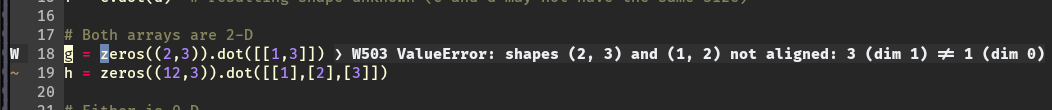
\includegraphics[width=\textwidth]{figures/neovim-linter.png}
\caption{Example of warning message displayed in (Neo)Vim as a result of checking the code
  with Pytropos.\label{pytroposlinter}}
\end{figure}

The required steps to use Pytropos as a linter in (Neo)Vim are:

\begin{itemize}
\tightlist
\item Install Pytropos and make sure it can be run from console.
\item Install the plugin Neomake. Homepage: \url{https://github.com/neomake/neomake}.
\item Tell Neomake how to interpret the Pytropos output by adding the following lines to
  the configuration file \verb|vimrc|:
  \begin{minted}[gobble=4]{vim}
    function! PostProcessingPytropos(entry)
        " Pytropos uses 0-indexed columns, and Neovim uses 1-indexed
        let a:entry.col += 1

        if a:entry.text =~# '^E'  ||  a:entry.text =~# '^SyntaxError'
            let a:entry.type = 'E'
        elseif a:entry.text =~# '^W'
            let a:entry.type = 'W'
        elseif a:entry.text =~# '^F'
            let a:entry.type = 'F'
        else
            let a:entry.type = 'A'
        endif
    endfunction

    let g:neomake_python_pytropos_maker = {
       \ 'exe': 'pytropos', " Change if Pytropos is called differently on your machine
       \ 'args': [],
       \ 'errorformat':
         \ '%f:%l:%c: %m',
      \ 'postprocess': [
         \ function('PostProcessingPytropos'),
         \ ]
      \ }

    let g:neomake_python_enabled_makers += ['pytropos']
  \end{minted}
\end{itemize}

\subsection*{Summary}

Pytropos is still at a very early stage of development. Its repeirtoire of Python
characteristics is still small (No support for \pycode|for| statement, custom classes and
objects, exception handling and the lack of builtin definitions). Nonetheless, Pytropos
can check for errors on operations between tensors and can be extended to work with more
libraries.

Pytropos is able to check for the many common cases and mistakes that can be made when
working with tensors. It is able to calculate the shape of tensors in a variety of
circumstances and can handle tricky or complex methods as the function \pycode|array| from
NumPy. The NumPy function \pycode|array| can evaluate almost anything as an array.
% Other libraries An example of why this is important can be seen in the library\todo{add
% ref to numpy mypy lib}.
